% Define document class
\documentclass[twocolumn]{aastex631}

% Custom style defs for this paper
\usepackage{listings}

\lstdefinestyle{bash}{%
    language=bash,
    basicstyle=\ttfamily\footnotesize,
    texcsstyle=*\bf\color{black},
    numbers=none,
    breaklines=true,
    commentstyle=\color{red},
    frame=single
}
\lstdefinestyle{yaml}{%
    basicstyle=\ttfamily\footnotesize,
    texcsstyle=*\bf\color{black},
    numbers=none,
    breaklines=true,
    commentstyle=\color{red},
    frame=single
}
\lstdefinestyle{LaTeX}{%
    language=[LaTeX]TeX,
    basicstyle=\ttfamily\footnotesize,
    texcsstyle=*\bf\color{black},
    numbers=none,
    breaklines=true,
    commentstyle=\color{red},
    frame=single,
    tabsize=2,
    keywords={begin,caption,label,end,includegraphics},   
}
\definecolor{lsthilite}{rgb}{0.0,0.0,1.0}

% Begin!
\begin{document}

% Title
\title{\showyourwork: a workflow for open source scientific articles}

% Author list
\author[0000-0002-0296-3826]{Rodrigo Luger}

% Abstract with filler text
\begin{abstract}
    Abstract coming soon.
\end{abstract}

% Main body with filler text
\section{Introduction}

Introduction coming soon.

\section{Starting a project}
\label{sec:start}
%
Users can start a new project by \href{https://github.com/rodluger/showyourwork-template/generate}{creating a fresh repository based on the \texttt{showyourwork-template}}.
This will create a new repository under the user's \texttt{GitHub} account and trigger a \texttt{GitHub Action} that will finish the setup process.
After a few minutes...
%
\begin{figure}[ht!]
    \begin{centering}
        
\includegraphics[width=\linewidth]{static/banner.png}
        \caption{
            The default \texttt{README} banner in a repository instantiated from the \texttt{showyourwork-template}, with links to the \texttt{GitHub Action} build logs, a tarball containing the \texttt{TeX} source for the article, a directed acyclic graph (DAG) of the build process, and the compiled article PDF, respectively.
        }
        \label{fig:banner}
    \end{centering}
\end{figure}
%

\section{Repository structure}
\label{sec:struct}
%
\begin{figure}[ht!]
    \begin{centering}
        \includegraphics[width=0.5\linewidth]{figures/tree.pdf}
        \caption{
            The basic repository structure for an open source scientfic article based on \texttt{showyourwork-template}.
            See text for details.
        }
        \label{fig:tree}
    \end{centering}
\end{figure}
%
Figure~\ref{fig:tree} shows the basic directory structure for a repository instantiated from \texttt{showyourwork-template}. 
The main components are:
\begin{itemize}
    \item \texttt{.github/workflow/showyourwork.yml}: The configuration file for the \texttt{GitHub Actions} workflow, with instructions on how to set up the virtual environment, checkout the repository, and invoke the \texttt{showyourwork-action} to build and publish the article PDF.
    \item \texttt{showyourwork}: The \texttt{git} submodule containing the \showyourwork workflow, which manages the entire build process for the article.
    \item \texttt{src}: A directory containing all of the scripts needed to generate the article.
    \item \texttt{src/data}: A directory containing programmatically generated (or downloaded) datasets and dependencies that are not tracked by \texttt{git}; this directory should be empty when the repository is first cloned.
    \item \texttt{src/figures}: A directory containing all of the scripts needed to generate the article figures.
    When the article is built, figure (output) files will be stored here, but they should not be tracked by \texttt{git}.
    \item \texttt{src/static}: A directory containing miscellaneous files (usually figures) that are tracked by \texttt{git}.
    These may include photographs, flowcharts, or other figures that cannot be programmatically generated.
    \item \texttt{src/ms.tex}: The main \texttt{TeX} article manuscript.
    \item \texttt{Makefile}: A read-only UNIX/Linux makefile that enables users to build the article by running \texttt{make} in the command-line terminal.
    \item \texttt{Snakefile}: A file containing the rules for the \texttt{Snakemake} workflow.
    By default, it simply imports all of the rules defined in \texttt{showyourwork/workflow/Snakefile}, but users can edit this file to add new rules or customize existing rules.
    \item \texttt{environment.yml}: The \texttt{conda} environment file specifying all of the direct software dependencies of the workflow.
    \item \texttt{showyourwork.yml}: The main configuration file for the workflow, where users can specify figure and dataset dependencies, instructions for downloading datasets from \texttt{Zenodo}, etc.
\end{itemize}

\section{Automatic figure generation}
\label{sec:auto-fig}
%
The workflow automatically determines the relationship between a figure (e.g., a \texttt{*.pdf} image) and the script that generated it (e.g., a \texttt{*.py} file) via inspection of the \texttt{figure} environment in the \texttt{TeX} file. 
Specifically, it inspects the \texttt{{\textbackslash}includegraphics} and \texttt{{\textbackslash}label} commands to infer the name of the figure and the script that generated it, respectively.
Consider the following snippet, used to generate Figure~\ref{fig:eccentricity}:
%
\begin{lstlisting}[
    style=LaTeX,
    otherkeywords={figures/eccentricity.pdf,fig:eccentricity},
    emph={figures/eccentricity.pdf,fig:eccentricity},
    emphstyle={\color{lsthilite}}
]
\begin{figure}
  \begin{centering}
    \includegraphics{figures/eccentricity.pdf}
    \caption{...}
    \label{fig:eccentricity}
  \end{centering}
\end{figure}
\end{lstlisting}
%
The convention in \showyourwork is to infer the parent script for a figure referenced in an \texttt{includegraphics} call (in this case, {\color{lsthilite}\texttt{figures/eccentricity.pdf}}) from the figure \texttt{label}. 
Specifically, if a label starts with {\color{lsthilite}\texttt{fig:}}, the remainder of the label (e.g., {\color{lsthilite}\texttt{eccentricity}}) is interpreted as the name of a script in the \texttt{figures/} directory which should be executed to produce that figure. 
By default, figure scripts are expected to be \texttt{Python} scripts, so in this case the workflow will attempt to run
%
\begin{lstlisting}[
    style=bash
]
python eccentricity.py
\end{lstlisting}
%
from within the \texttt{figures/} directory to generate \texttt{eccentricity.pdf}.

This behavior may be customized in several ways. 
First, the figure script need not be a \texttt{Python} script; see \S\ref{sec:other-lang} for information on how to include scripts in any language.
Second, a common scenario involves a script that generates multiple figures.
These can all be included (using \texttt{includegraphics}) in the same figure environment with a single shared label (denoting the name of the script)
...

\section{Support for other languages}
\label{sec:other-lang}
%
Scripts in languages other than \texttt{Python} are supported via the inclusion of entries under the \texttt{scripts} key in the \texttt{showyourwork.yml} config file. 
Consider Figure~\ref{fig:tree}, which was generated from the \texttt{TeX} file \texttt{figures/tree.tex}, which contains a \texttt{TikZ} picture. 
In the main manuscript, we include the figure in the usual way, i.e.,
%
\begin{lstlisting}[
    style=LaTeX,
    otherkeywords={figures/eccentricity.pdf,fig:eccentricity},
    emph={figures/eccentricity.pdf,fig:eccentricity},
    emphstyle={\color{lsthilite}}
]
\begin{figure}
  \begin{centering}
    \includegraphics{figures/tree.pdf}
    \caption{...}
    \label{fig:tree}
  \end{centering}
\end{figure}
\end{lstlisting}
%
By default, as we saw in \S\ref{sec:auto-fig}, this instructs the workflow to execute a file called \texttt{figures/tree.py} to generate the corresponding figure. 
However, in the present case, that file does not exist; instead, we have a file called \texttt{figures/tree.tex}, which we would like to compile into a \texttt{PDF} using te \texttt{tectonic} engine.
We can instruct the workflow to do this by specifying the following in \texttt{showyourwork.yml}:
%
\begin{lstlisting}[
    style=yaml,
    otherkeywords={script.path,script.name},
    emph={script.path,script.name},
    emphstyle={\color{lsthilite}}
]
scripts:
  tex:
    cd {script.path} && tectonic {script.name}
\end{lstlisting}
%
Each entry under the \texttt{scripts} key should be a file extension, and under each one, a string containing a shell command that instructs the workflow how to execute a given {\color{lsthilite}\texttt{script}} to produce a given {\color{lsthilite}\texttt{output}}.
For convenience, the following placeholders are recognized and expand as follows at runtime:
%
\begin{itemize}
\item \texttt{\{script\}}: The full path to the input script.
\item \texttt{\{script.path\}}: The full path to the directory containing the input script.
\item \texttt{\{script.name\}}: The name of the input script (without the path).
\item \texttt{\{output\}}: The full path to the output file.
\item \texttt{\{output.path\}}: The full path to the directory containing the output file.
\item \texttt{\{output.name\}}: The name of the output file (without the path).
\end{itemize}
%
If additional customization is needed, such as the need to provide command-line arguments that are specific to individual figures, users should instead provide custom rules in the \texttt{Snakefile} (\S\ref{sec:arbitrary-rules}).

\section{Arbitrary rules}
\label{sec:arbitrary-rules}
%
Coming soon.

\begin{figure}[ht!]
    \begin{centering}
        \includegraphics[width=\linewidth]{figures/eccentricity.pdf}
        \caption{
            The effect of eccentricity on the detectability of a \emph{LISA} source; reproduced from Figure 3 in \citet{Wagg2021}.
        }
        \label{fig:eccentricity}
    \end{centering}
\end{figure}

\begin{figure}[ht!]
    \begin{centering}
        \includegraphics[width=\linewidth]{figures/luhman16b.pdf}
        \caption{
            16 \emph{CRIRES} spectra of WISE 1049-5319B spanning a full rotation period of the brown dwarf; adapted from Figure 14 in \citet{Luger2021}. 
            Data originally from \citet{Crossfield2014}.
        }
        \label{fig:luhman16b}
    \end{centering}
\end{figure}

\begin{figure}[ht!]
    \begin{centering}
        \includegraphics[width=\linewidth]{figures/rossbyridge.pdf}
        \caption{
            A pile-up of stars in the rotation period-temperature space at slightly faster rotation than the sun (orange dot); adapted from Figure 1 in David et al. (in prep).
        }
        \label{fig:rossbyridge}
    \end{centering}
\end{figure}

\begin{figure}[ht!]
    \begin{centering}
        \includegraphics[width=\linewidth]{figures/HD118203_transit.pdf}
        \includegraphics[width=\linewidth]{figures/HD118203_corner.pdf}
        \caption{
            The phase-folded transit of HD 118203b in \emph{TESS} (\emph{top}) and the inferred joint posterior distributions over its period, radius, and impact parameter (\emph{bottom}); adapted from the \texttt{exoplanet} documentation \citep{ForemanMackey2021}.
            Both figures were generated from the same \texttt{Python} script in the \texttt{src/figures} directory (linked to in the \texttt{GitHub} icon in the margin). The other margin icon indicates that these figures depend on a dataset (a \texttt{.npz} file containing the posterior samples), which is automatically generated by \showyourwork and uploaded to Zenodo. 
            Users wishing to reproduce the results in this paper can choose whether to re-generate this dataset or download a static version from Zenodo (linked to in the margin).
        }
        \label{fig:HD118203}
    \end{centering}
\end{figure}

\begin{figure}[ht!]
    \begin{centering}
        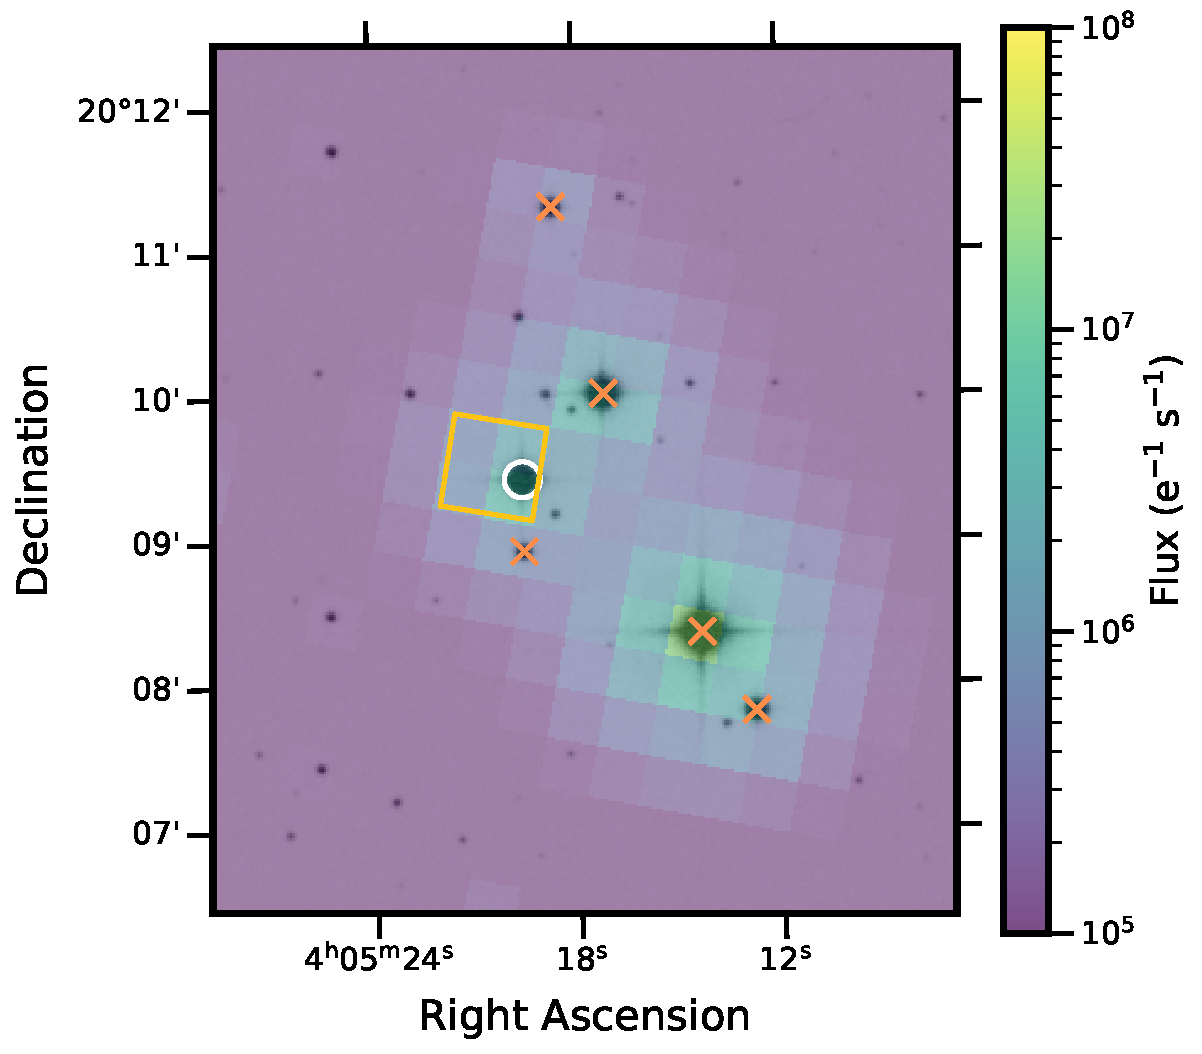
\includegraphics[width=\linewidth]{static/TESSaperture.pdf}
        \caption{
            \emph{TESS} target pixel file (TPF) of V1298 Tau
            overlaid with an r-band sky image from the Digitized Sky Survey (DSS);
            reproduced from Figure 1 in \citet{Feinstein2021}.
            This figure exists as a static PDF, with no associated script to
            generate it.
            We therefore include it in the \texttt{src/static} directory, which tells \showyourwork to not attempt to generate it. 
            By default, margin icons are not added to static figures.
            Here we manually add an icon linking to the original paper using the \texttt{\textbackslash marginicon} command.
        }
        \marginicon{%
            \href{https://ui.adsabs.harvard.edu/abs/2021arXiv211108660F}{\color{sywBlue}\faNewspaper[regular]}
        }
        \label{fig:eclipse}
    \end{centering}
\end{figure}

\begin{figure*}[ht!]
    \begin{centering}
        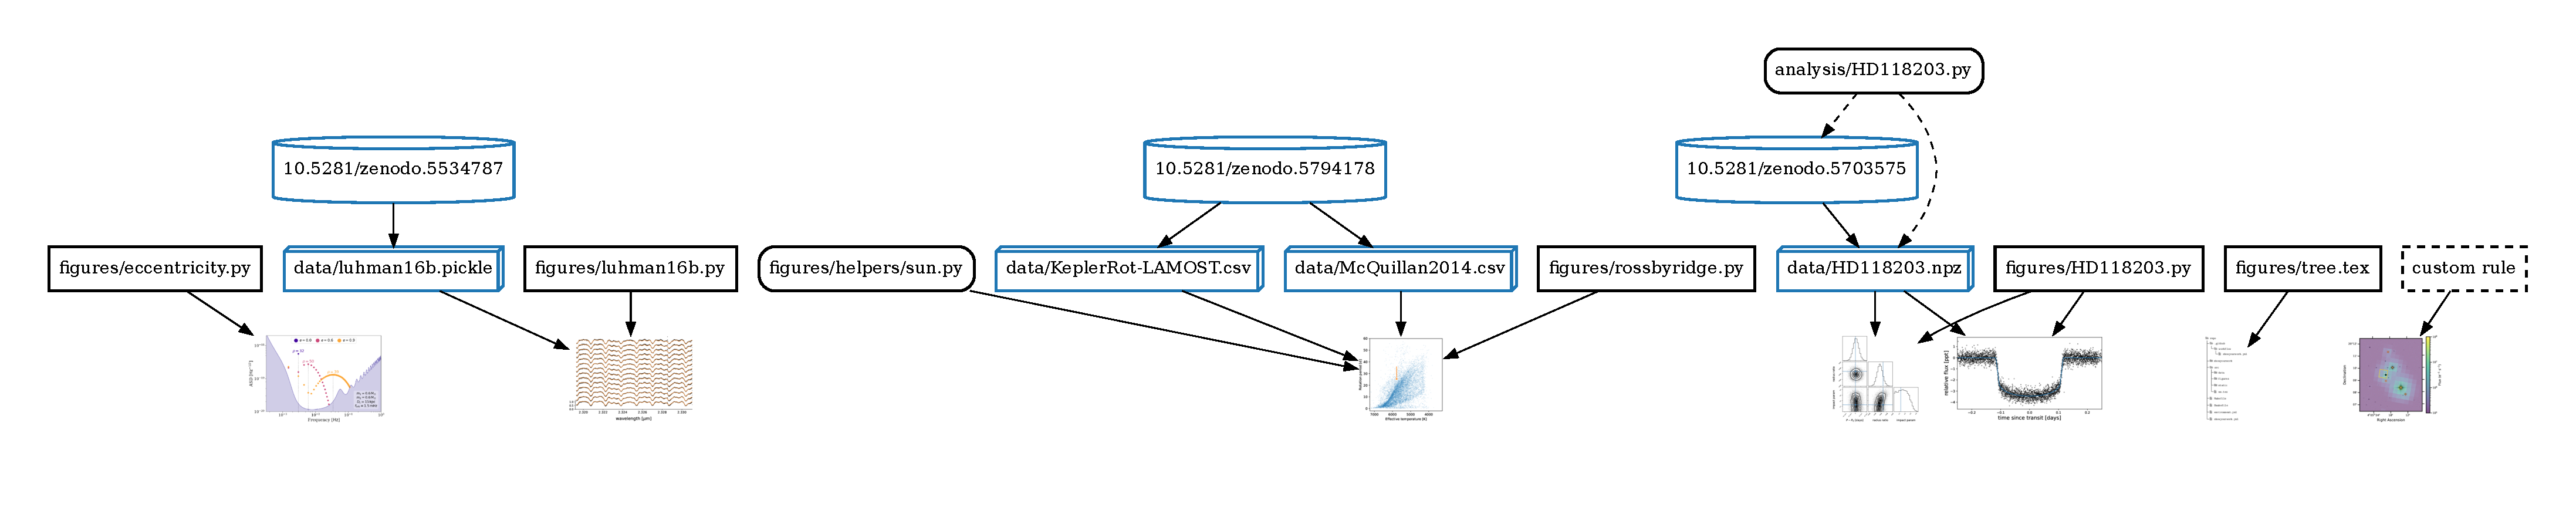
\includegraphics[width=\linewidth]{figures/dag.pdf}
        \caption{
            A directed acyclic graph (DAG) showing the build process for each of the (other) figures in this article. 
            Figure scripts are represented by black rectangles; helper scripts (such as ones imported by figure scripts or used in dataset generation) are similar, but have rounded edges.
            Blue cylinders correspond to Zenodo records; blue boxes correspond to datasets.
        }
        \label{fig*:dag}
    \end{centering}
\end{figure*}

\bibliography{bib}

\end{document}
